\documentclass[12pt]{article}
\usepackage{natbib}
\usepackage{url}
\usepackage{fullpage}

\usepackage{times}

\usepackage{graphicx}
\usepackage{float}
\usepackage{capt-of}
\usepackage{subcaption}

\begin{document}
\title{Reflection Space Image Based Environment Mapping}
\author{Kyung yul Kevin Lim, Myron Liu}
\date{\today}
\maketitle

\section{Abstract}
We implement Reflection Space Image Based Rendering as described by Cabral et al.\cite{cabral1999reflection}. The goal is to generate a scene in which the user can rotate around the object lit by an HDR environment map, and observe view dependent BRDF changes in real time.

\section{Results}
\begin{figure}[H]
\centering
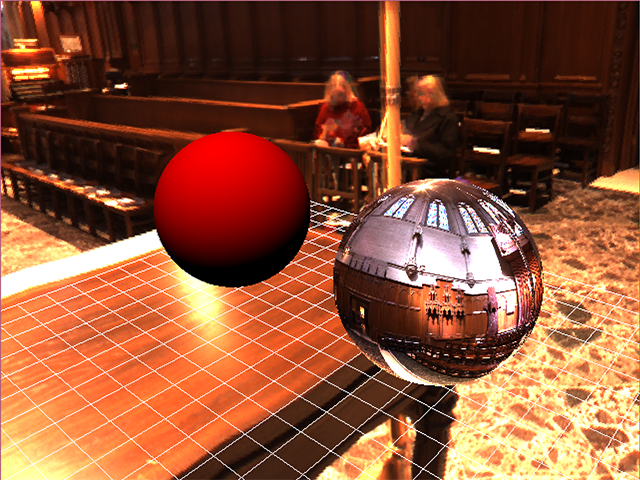
\includegraphics[width=0.75\textwidth]{{Figures/Milestone.png}}
\caption{A diffuse sphere and a fully mirrored sphere} 
\label{fig:milestone}
\end{figure}

\section{Current Progress}


Right now we are working primarily on shading a perfectly reflective sphere. We already have a framework established for grabbing the camera position at each instant, and using that camera position, along with the fragment position and fragment vector to compute the reflection direction $(\theta,\phi)$. From this, we can grab the relevant texture via the simple formula given on http://gl.ict.usc.edu/Data/HighResProbes/, which is the source from which our HDR image originates. It's not really working quite as intended; it looks more like the texture is simply wrapped onto the sphere, and the texture doesn't change with the viewing direction.

Regarding shading diffuse surfaces, we have set up a framework for integrating the environment map over a hemisphere oriented along the surface normal. We naively shaded a sphere using a uniform light source, but soon, we will swap this out for light coming in from every direction, as is the case with environment maps

%\bibliographystyle{plain}
%\bibliography{MilestoneReport}

\end{document}

